% -*- Mode:LaTeX -*-

\documentclass[twocolumn,prl,superscriptaddress]{revtex4}

% Required packages
\usepackage{dcolumn}
\usepackage{amsmath}
%\usepackage{calrsfs}

% Optional extra packages
\usepackage{graphicx}
\usepackage{subfigure}

% Can delete this at the end
\usepackage{comment}

% Style parameters
\setlength{\parskip}{0pt}
\setlength{\tabcolsep}{6pt}
\setlength{\arraycolsep}{2pt}

% Macros

\newcommand{\dd}{\mathrm{d}}
\newcommand{\ii}{\mathrm{i}}
\newcommand{\e}{\mathrm{e}}
\newcommand{\half}{\tfrac12}
\newcommand{\set}[1]{\lbrace#1\rbrace}
\newcommand{\av}[1]{\left\langle#1\right\rangle}
\newcommand{\etal}{{\it{}et~al.}}
\newcommand{\defn}{\textit}
\newcommand{\Ord}{\mathrm{O}}
\newcommand{\Tr}{\mathop\mathrm{Tr}}
\newcommand{\erf}{\mathop\mathrm{erf}}
\renewcommand{\Im}{\mathop\mathrm{Im}}
\newcommand{\mat}{\mathbf}
\renewcommand{\vec}{\mathbf}
\newcommand\Beta{\mathrm{B}}

\newcommand\pin{p_\textrm{in}}
\newcommand\pout{p_\textrm{out}}
\newcommand\cin{c_\textrm{in}}
\newcommand\cout{c_\textrm{out}}


\begin{document}

\title{An improved eigenvector centrality based on the non-backtracking matrix}
\author{Travis Martin}
\affiliation{Department of Electrical Engineering and Computer Science,
  University of Michigan, Ann Arbor, MI 48109}
\author{Xiao Zhang}
\affiliation{Department of Physics, University of Michigan, Ann Arbor, MI 48109}
\author{M. E. J. Newman}
\affiliation{Department of Physics and Center for the Study of Complex Systems, University of Michigan, Ann Arbor, MI 48109}

\begin{abstract}
  We show that eigenvector centrality behaves poorly on sparse random networks with vertices of unusually high degree, or hubs. We give numerical and analytical evidence that traditional eigenvector centrality is susceptible to localization, giving disproportionately high centrality to hubs and their neighbors. We propose an alternative centrality measure, \emph{non-backtracking centrality}, which converges to eigenvector centrality for dense networks and avoids the problem of localization around hubs in sparse networks.
\end{abstract}

\maketitle

Network researchers have long been interested in an effective method of measuring \emph{centrality}, a quantification of how important or central each network node is. Eigenvector centrality~\cite{bonacich72} is among the most influential centrality measures, with widely ranging applications to metabolic networks~\cite{ding10}, football team ranking~\cite{keener93}, bird mating analysis~\cite{ryder08}, and Google's highly successful PageRank algorithm\footnote{PageRank uses a closely related variant of eigenvector centrality}~\cite{brin98}. Eigenvector centrality specifies that each node's centrality be proportional to the sum of its neighbor's centralities, and can be conveniently calculated from the leading eigenvector of the network's adjacency matrix. Chung~\etal show that the largest eigenvalue of the adjacency matrix of a random graph model is almost surely determined by the larger of the square root of the maximum degree, $\sqrt{m}$, and the weighted average of the squares of the expected degrees, $\tilde{d}$~\cite{chung03}. In this paper we show that, at least for the Poisson with planted hub and power law random graph families, eigenvector centrality fails when the leading eigenvalue corresponds to $\sqrt{m}$ by giving a centrality vector which is too-localized around the highest degree node. In the second half of this paper we introduce \emph{non-backtracking centrality}, calculated from an alternative network representation called the non-backtracking matrix~\cite{krzakala13} or Hashimoto edge matrix~\cite{hashimoto89}, which avoids this failure case of eigenvector centrality while remaining asymptotically equal in the dense limit.

We first consider the Poisson random graph with nodes of identical expected degree $c$ and a planted hub of expected degree $k_n$. In Fig.~\ref{fig:transition} we display eigenvector (left column) and non-backtracking (right column) centralities for the hub and all nodes within distance 2, from the same Poisson random graph with size $n=1000000$ and $c = 10$. The rows show increasing hub size, from $k_n = 20$, $k_n = 70$, and $k_n = 120$. The eigenvector centralities, which are proportional to node areas, increase dramatically from $k_n = 70$ to $k_n = 120$ while the non-backtracking centralities increase steadily. We demonstrate below that this sudden increase in centrality is an undesirable side-effect of a phase transition in the leading eigenvalue.

Nadakuditi and Newman give careful analysis of the spectrum of a Poisson random graph with a planted hub~\cite{nadakuditi13}, and show the presence of an eigenvalue corresponding to the average degree at $c+1$ and an eigenvalue corresponding to the hub at $k_n / \sqrt{k_n - c}$. Setting these equal to each other and solving for $k_n$, we see that the hub eigenvalue overtakes the average degree eigenvalue at
\begin{equation}
k_n = c(c+1)
\end{equation}

%talk about global vs local??

\begin{figure}
\begin{center}
        %\subfigure{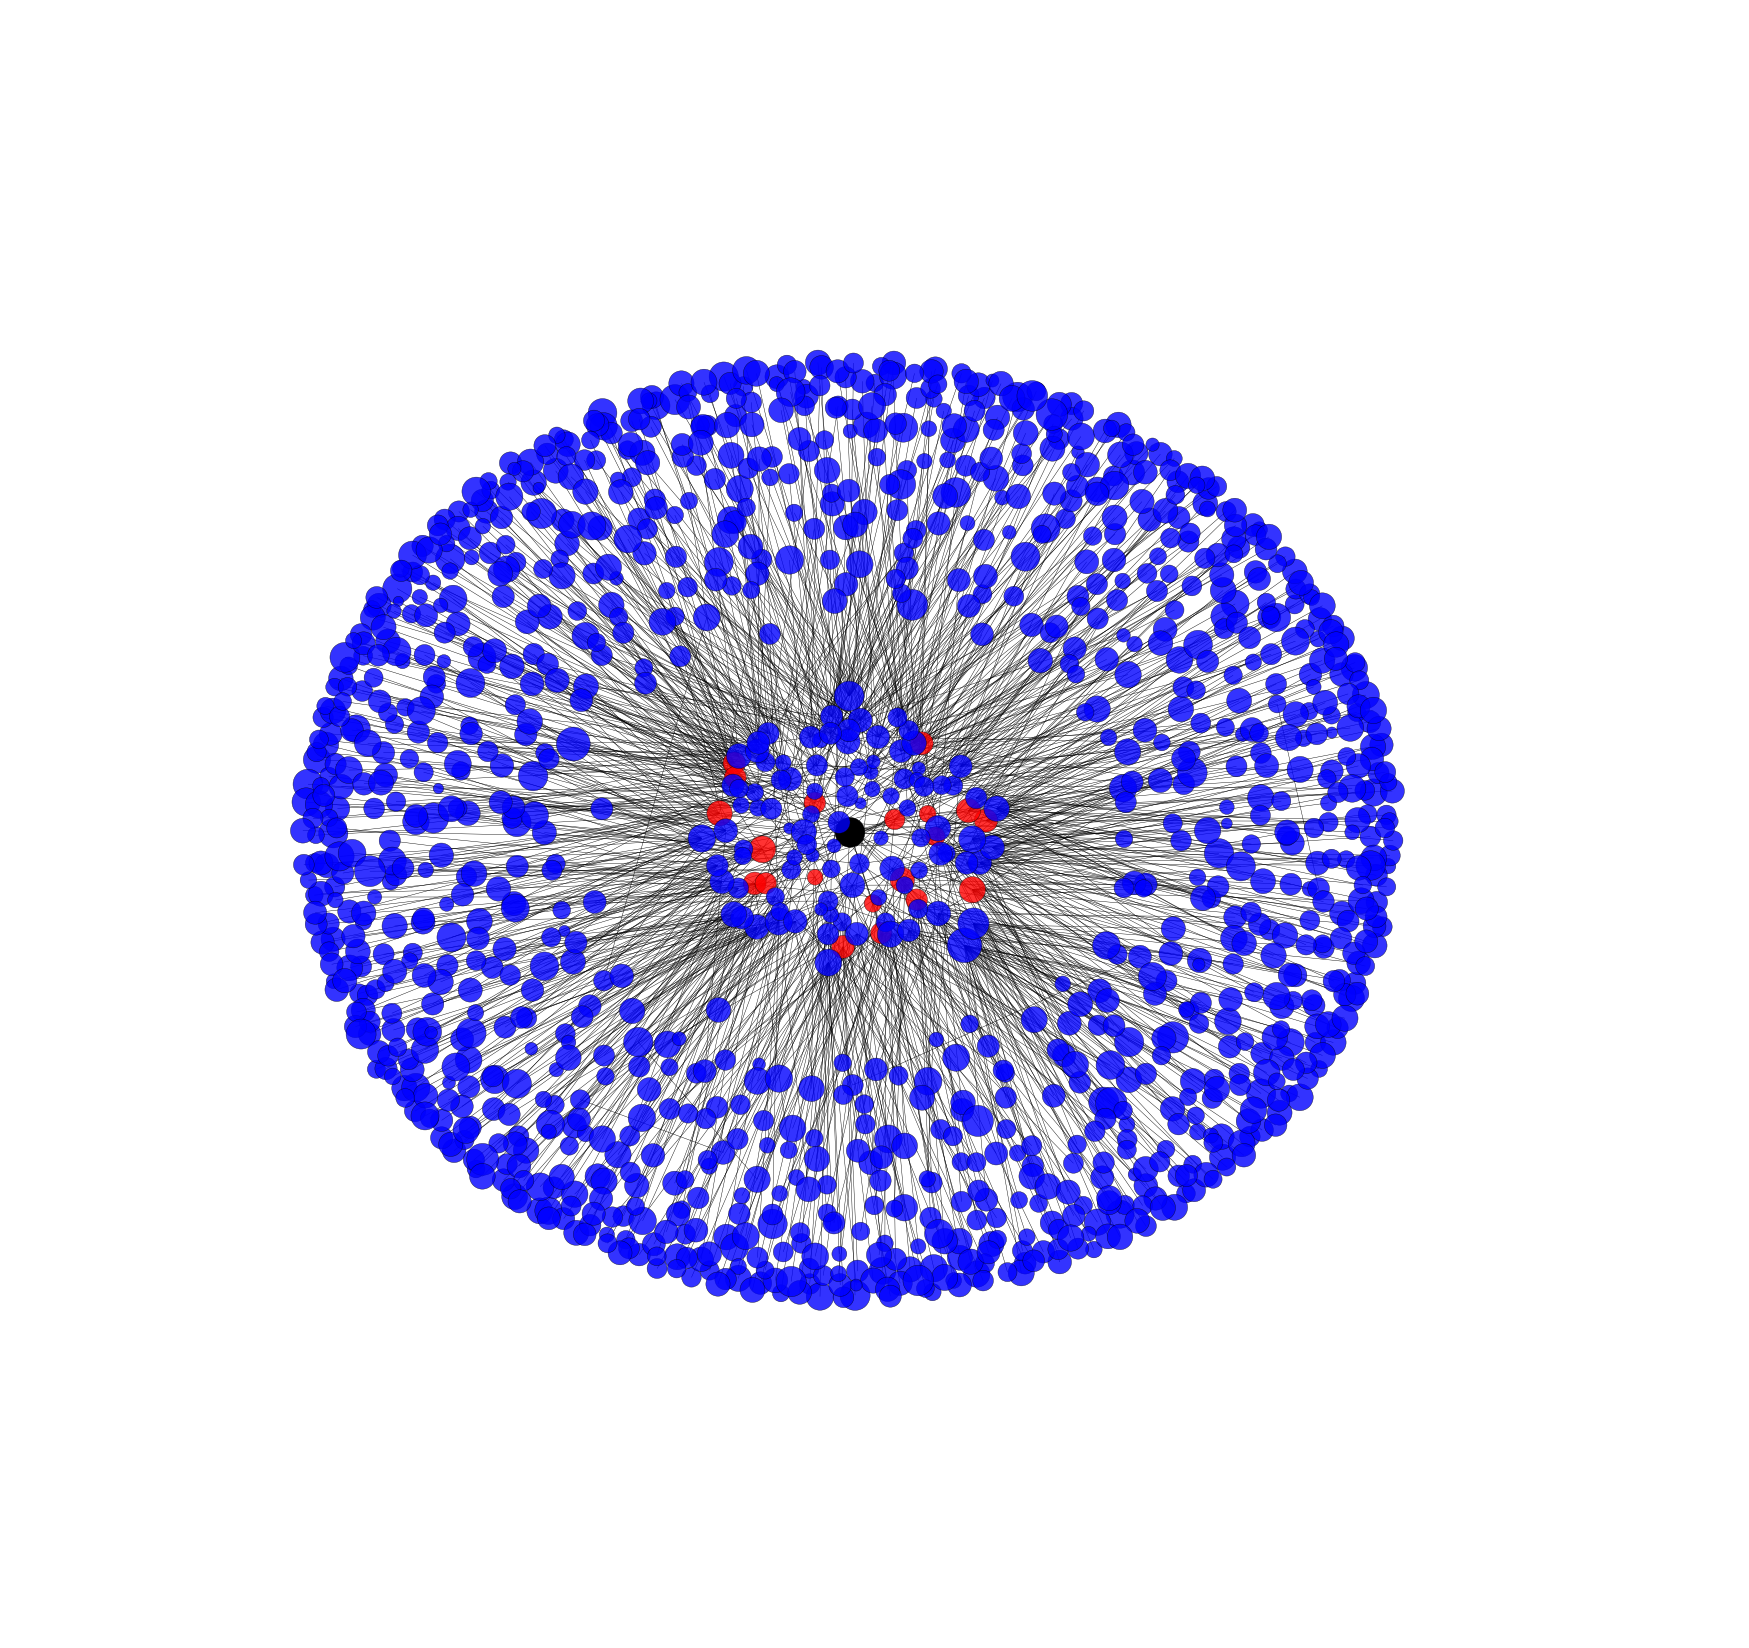
\includegraphics[width=0.49\columnwidth]{1.png}}
        %\subfigure{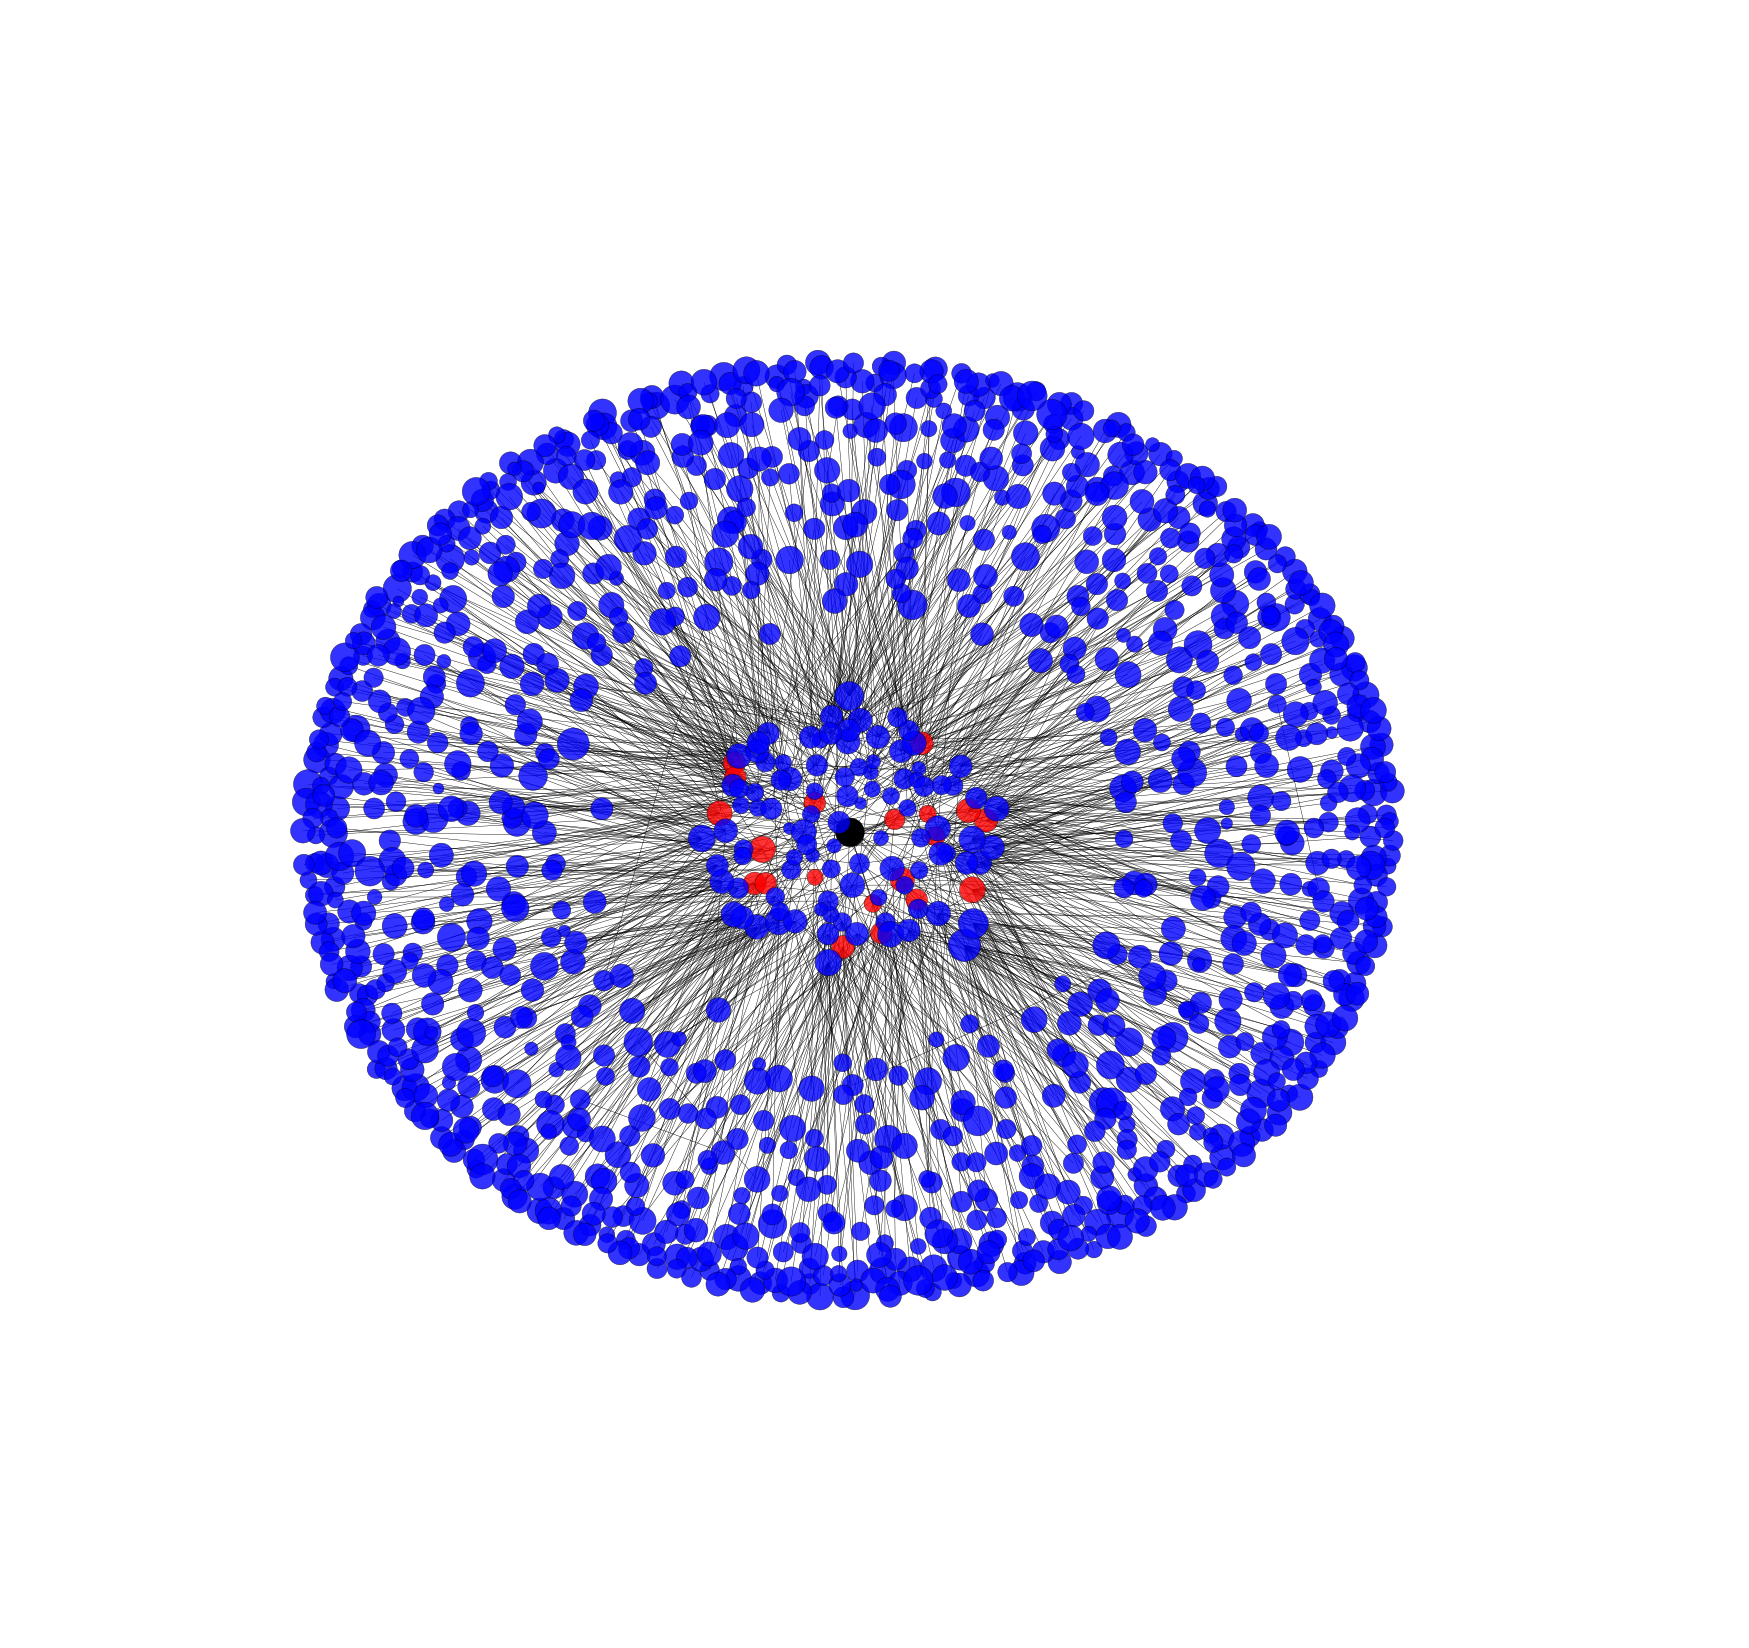
\includegraphics[width=0.49\columnwidth]{1h.png}}
        %\subfigure{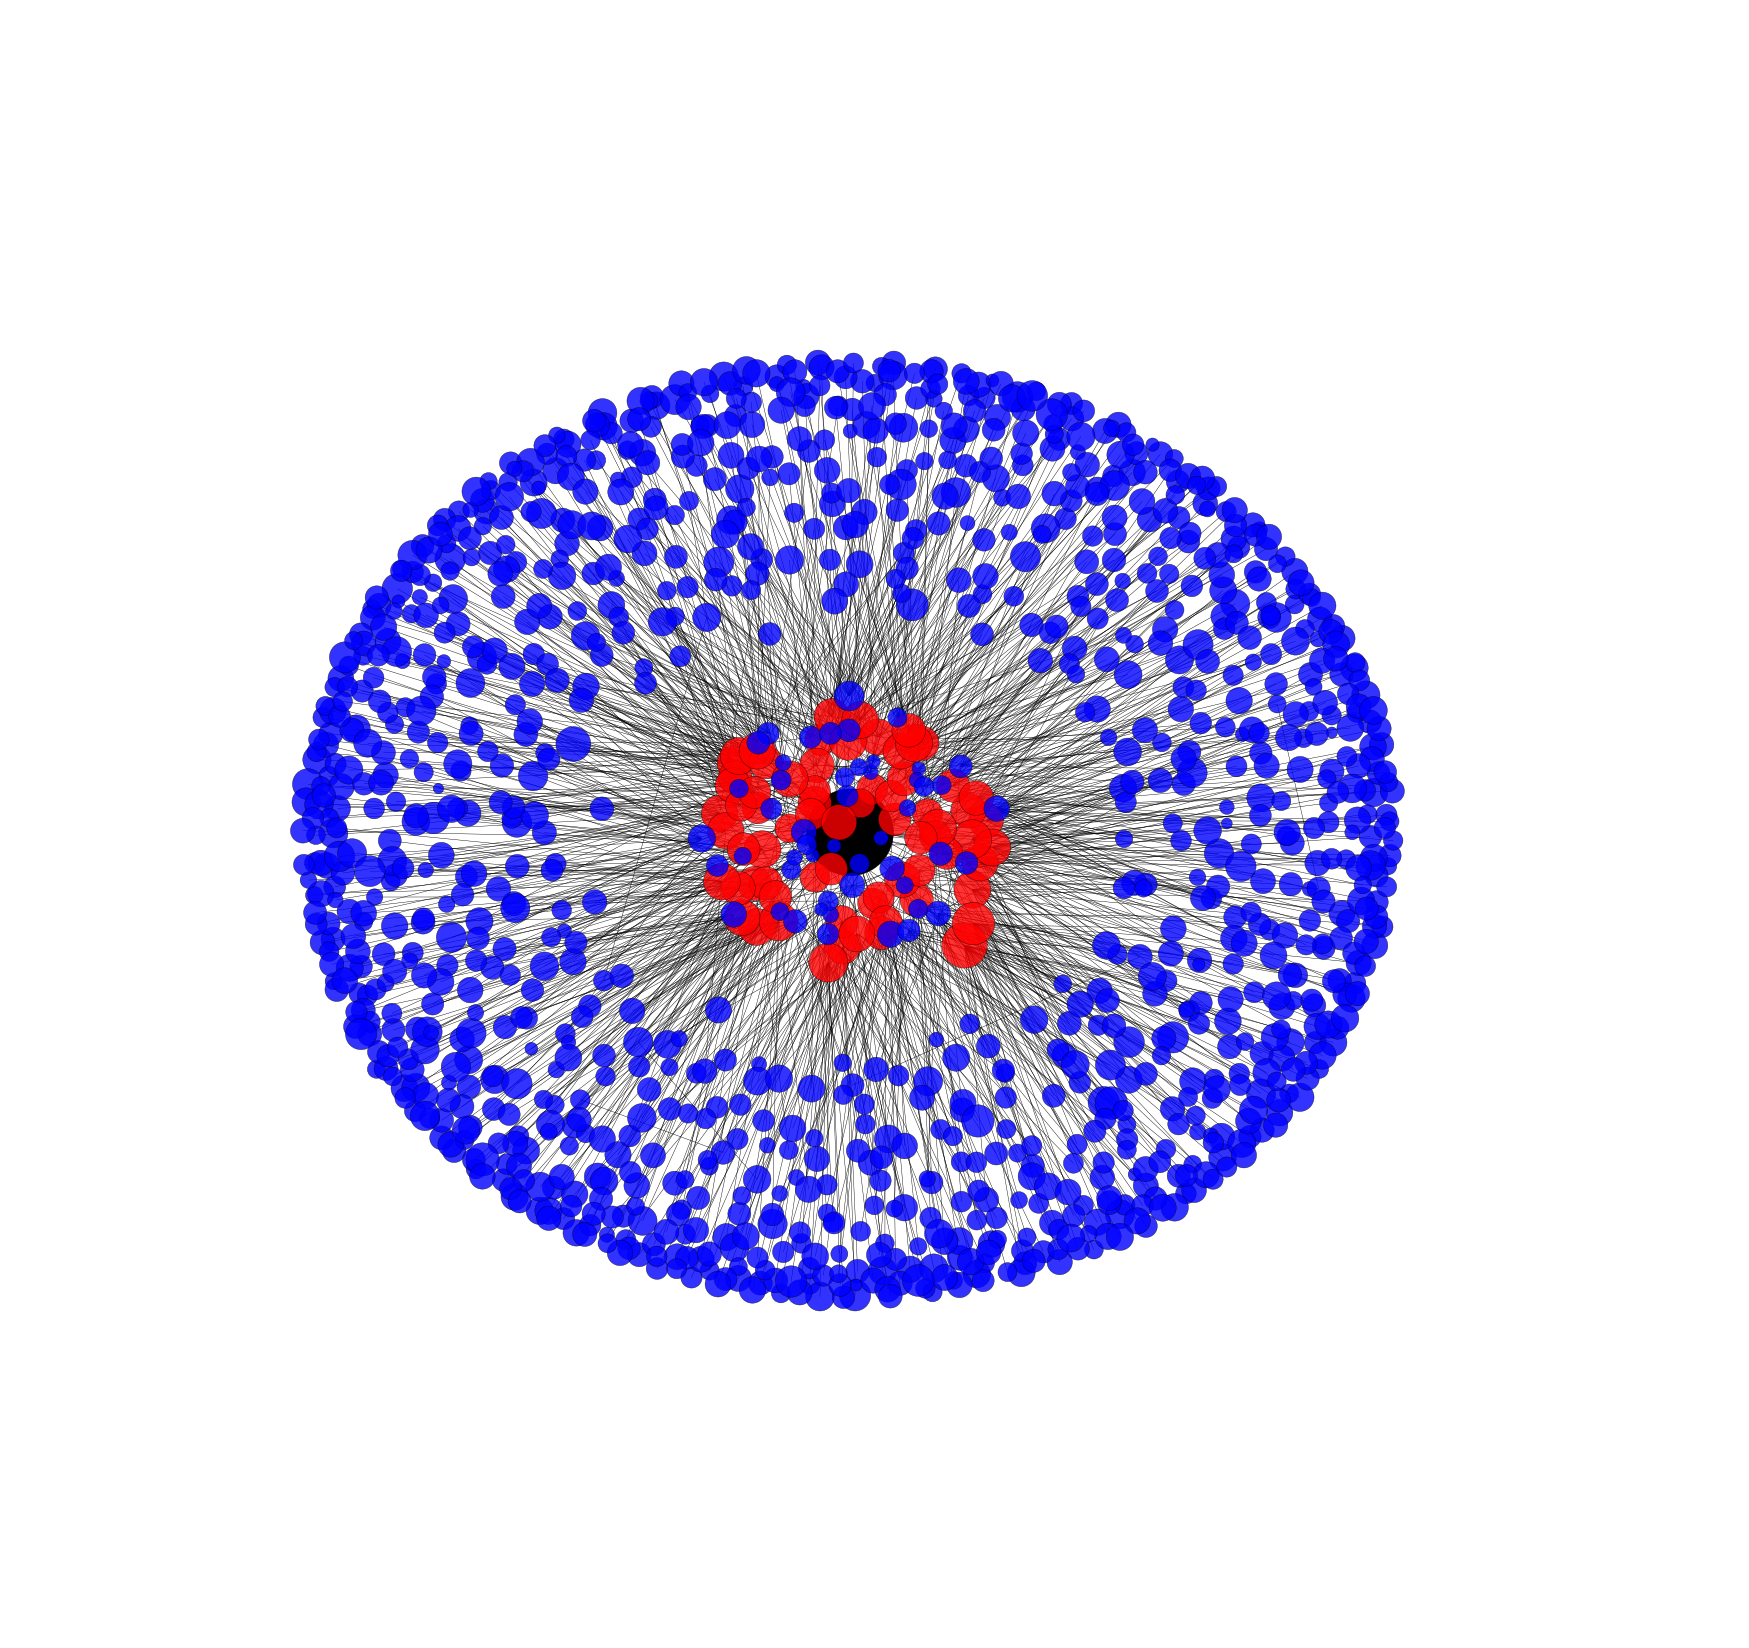
\includegraphics[width=0.49\columnwidth]{2.png}}
        %\subfigure{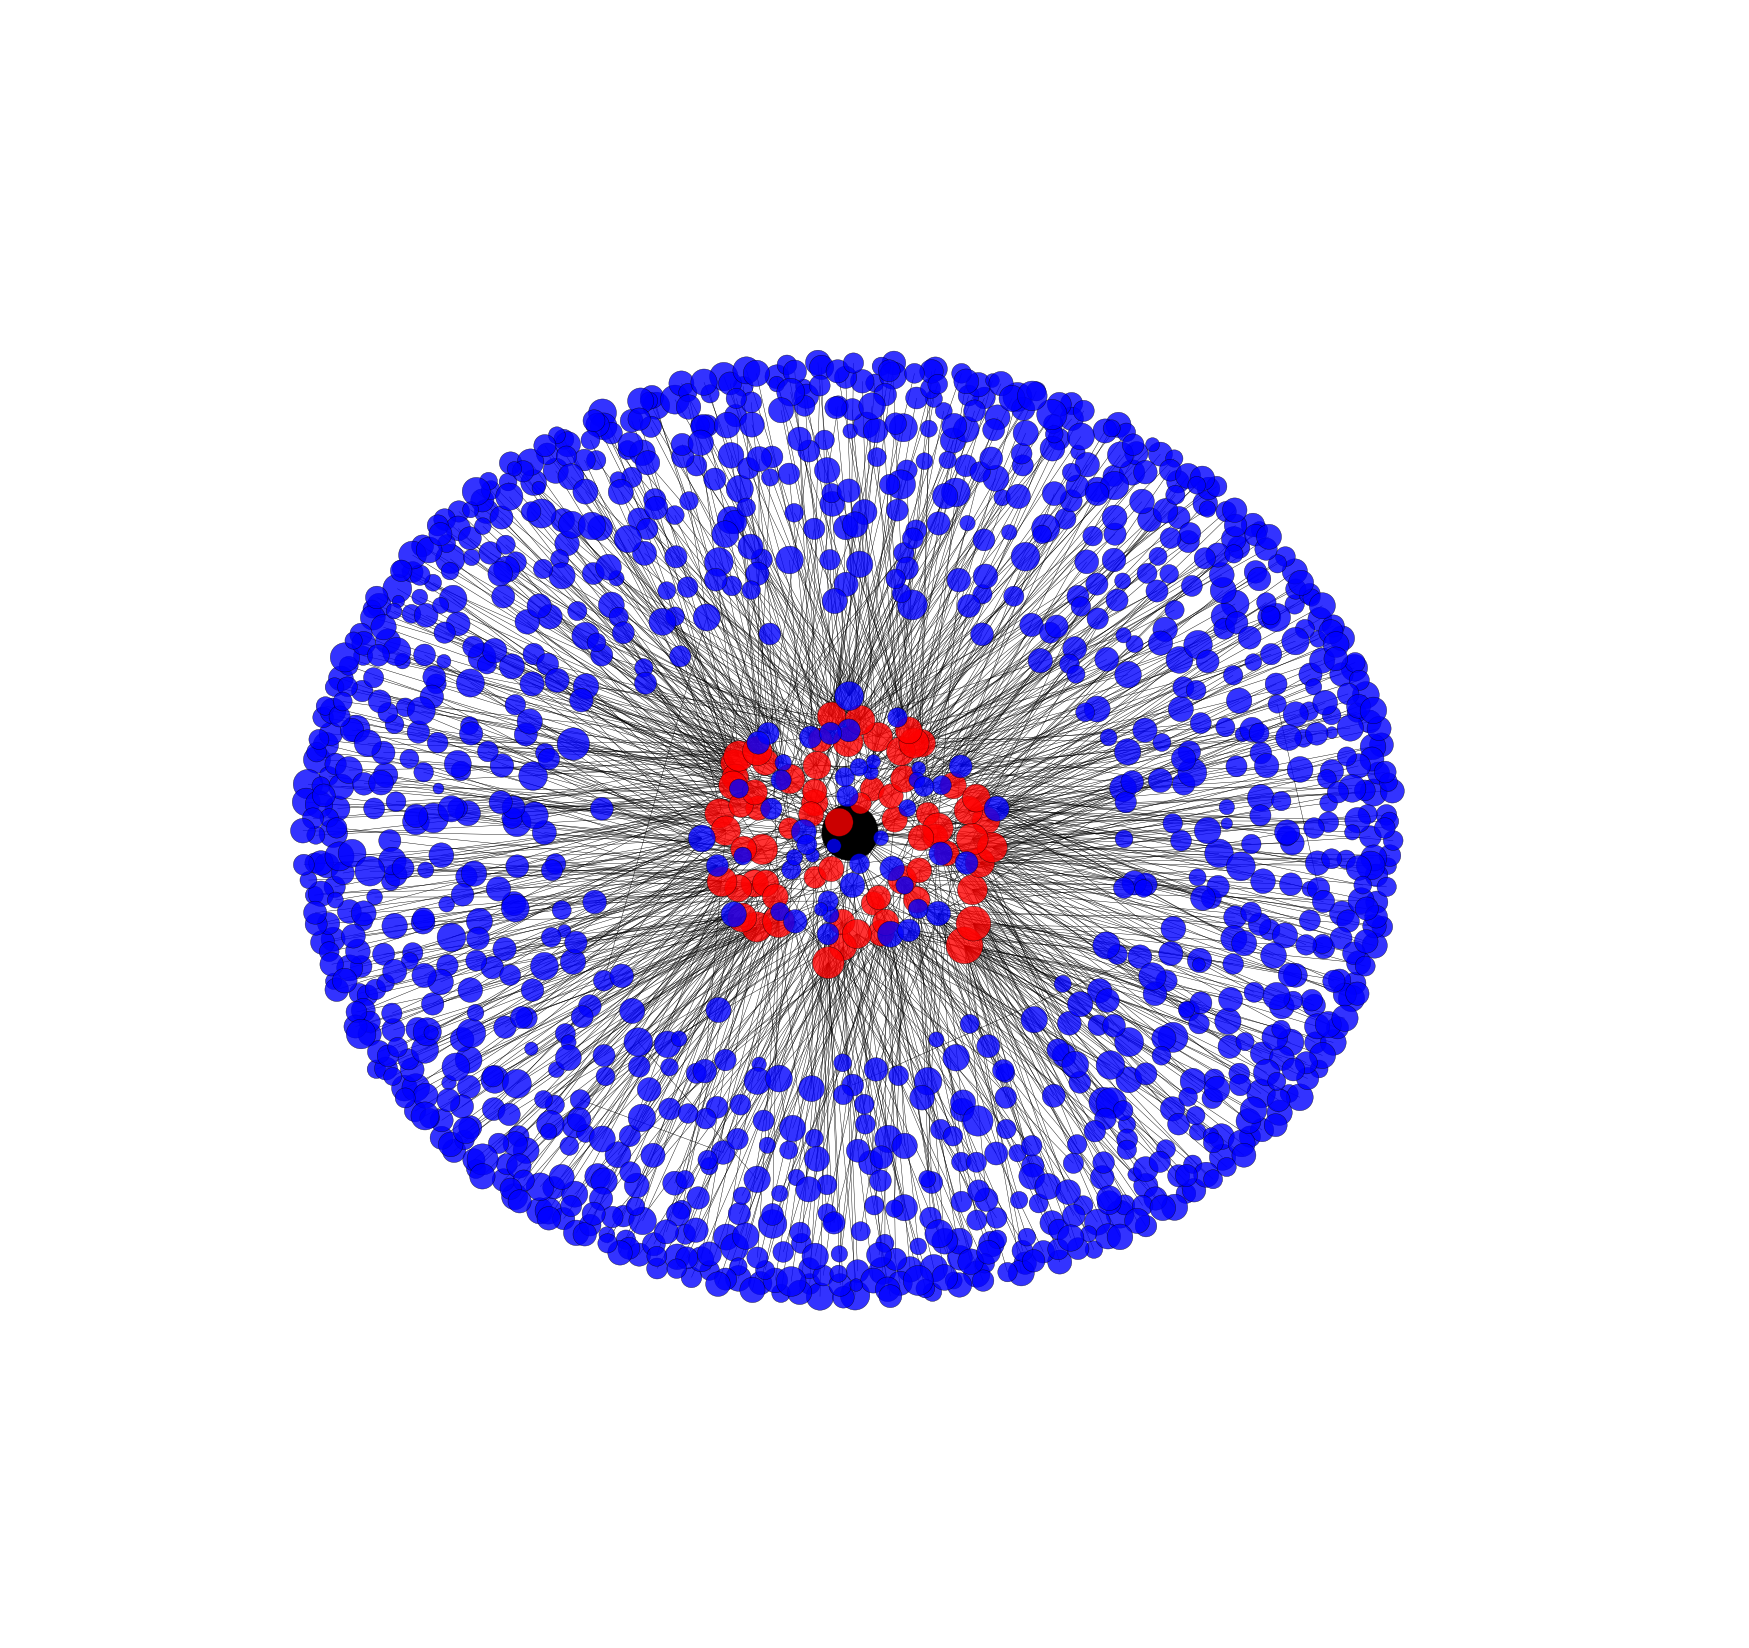
\includegraphics[width=0.49\columnwidth]{2h.png}}
        %\subfigure{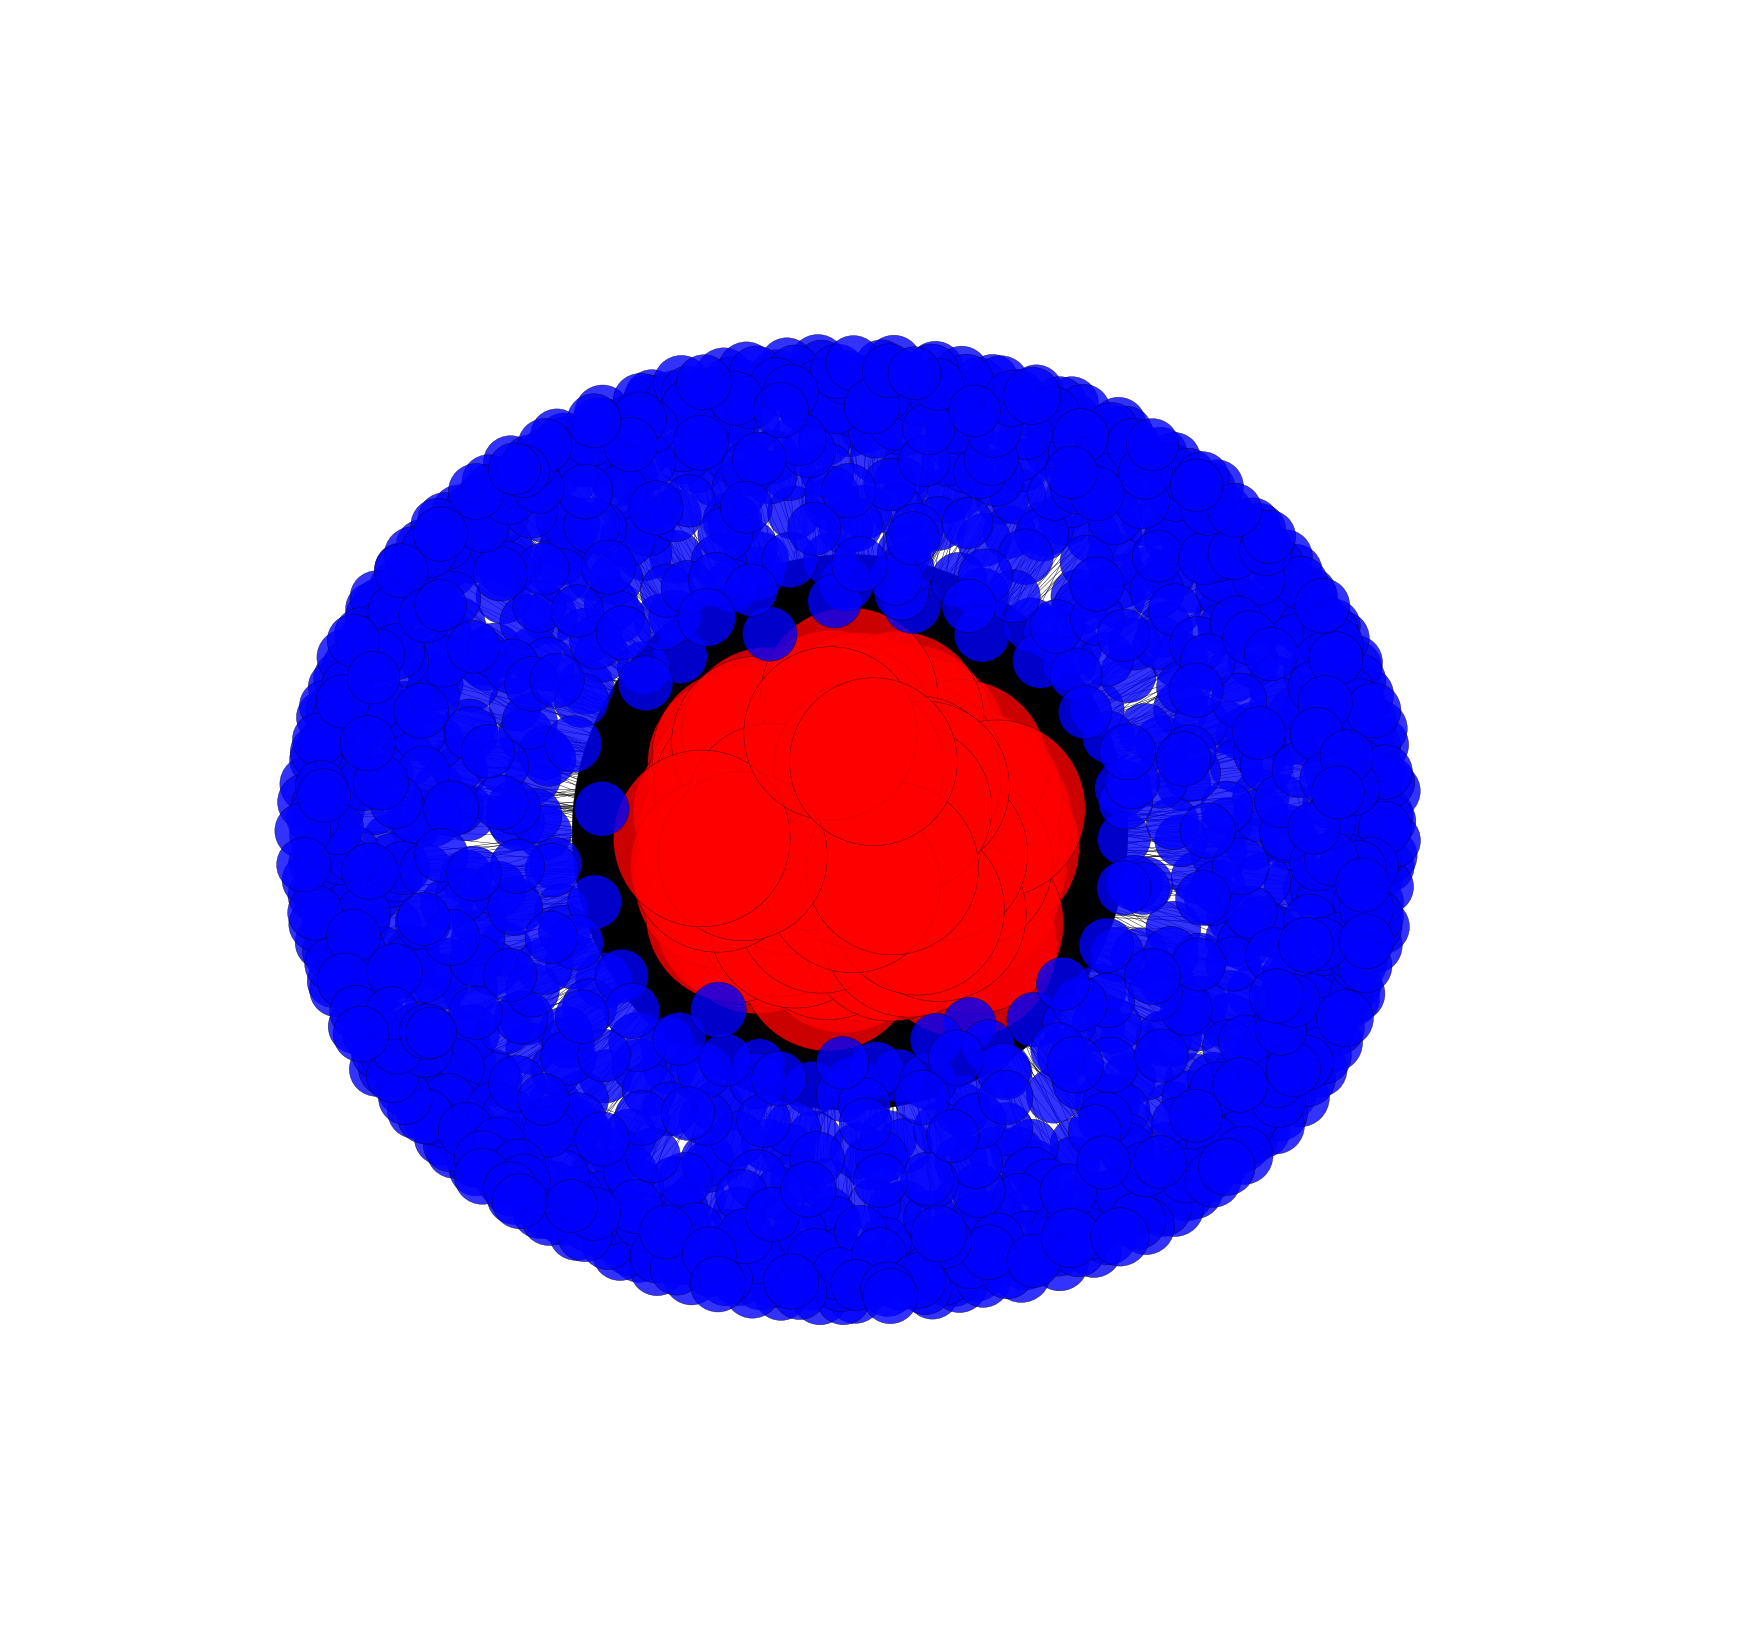
\includegraphics[width=0.49\columnwidth]{3.png}}
        %\subfigure{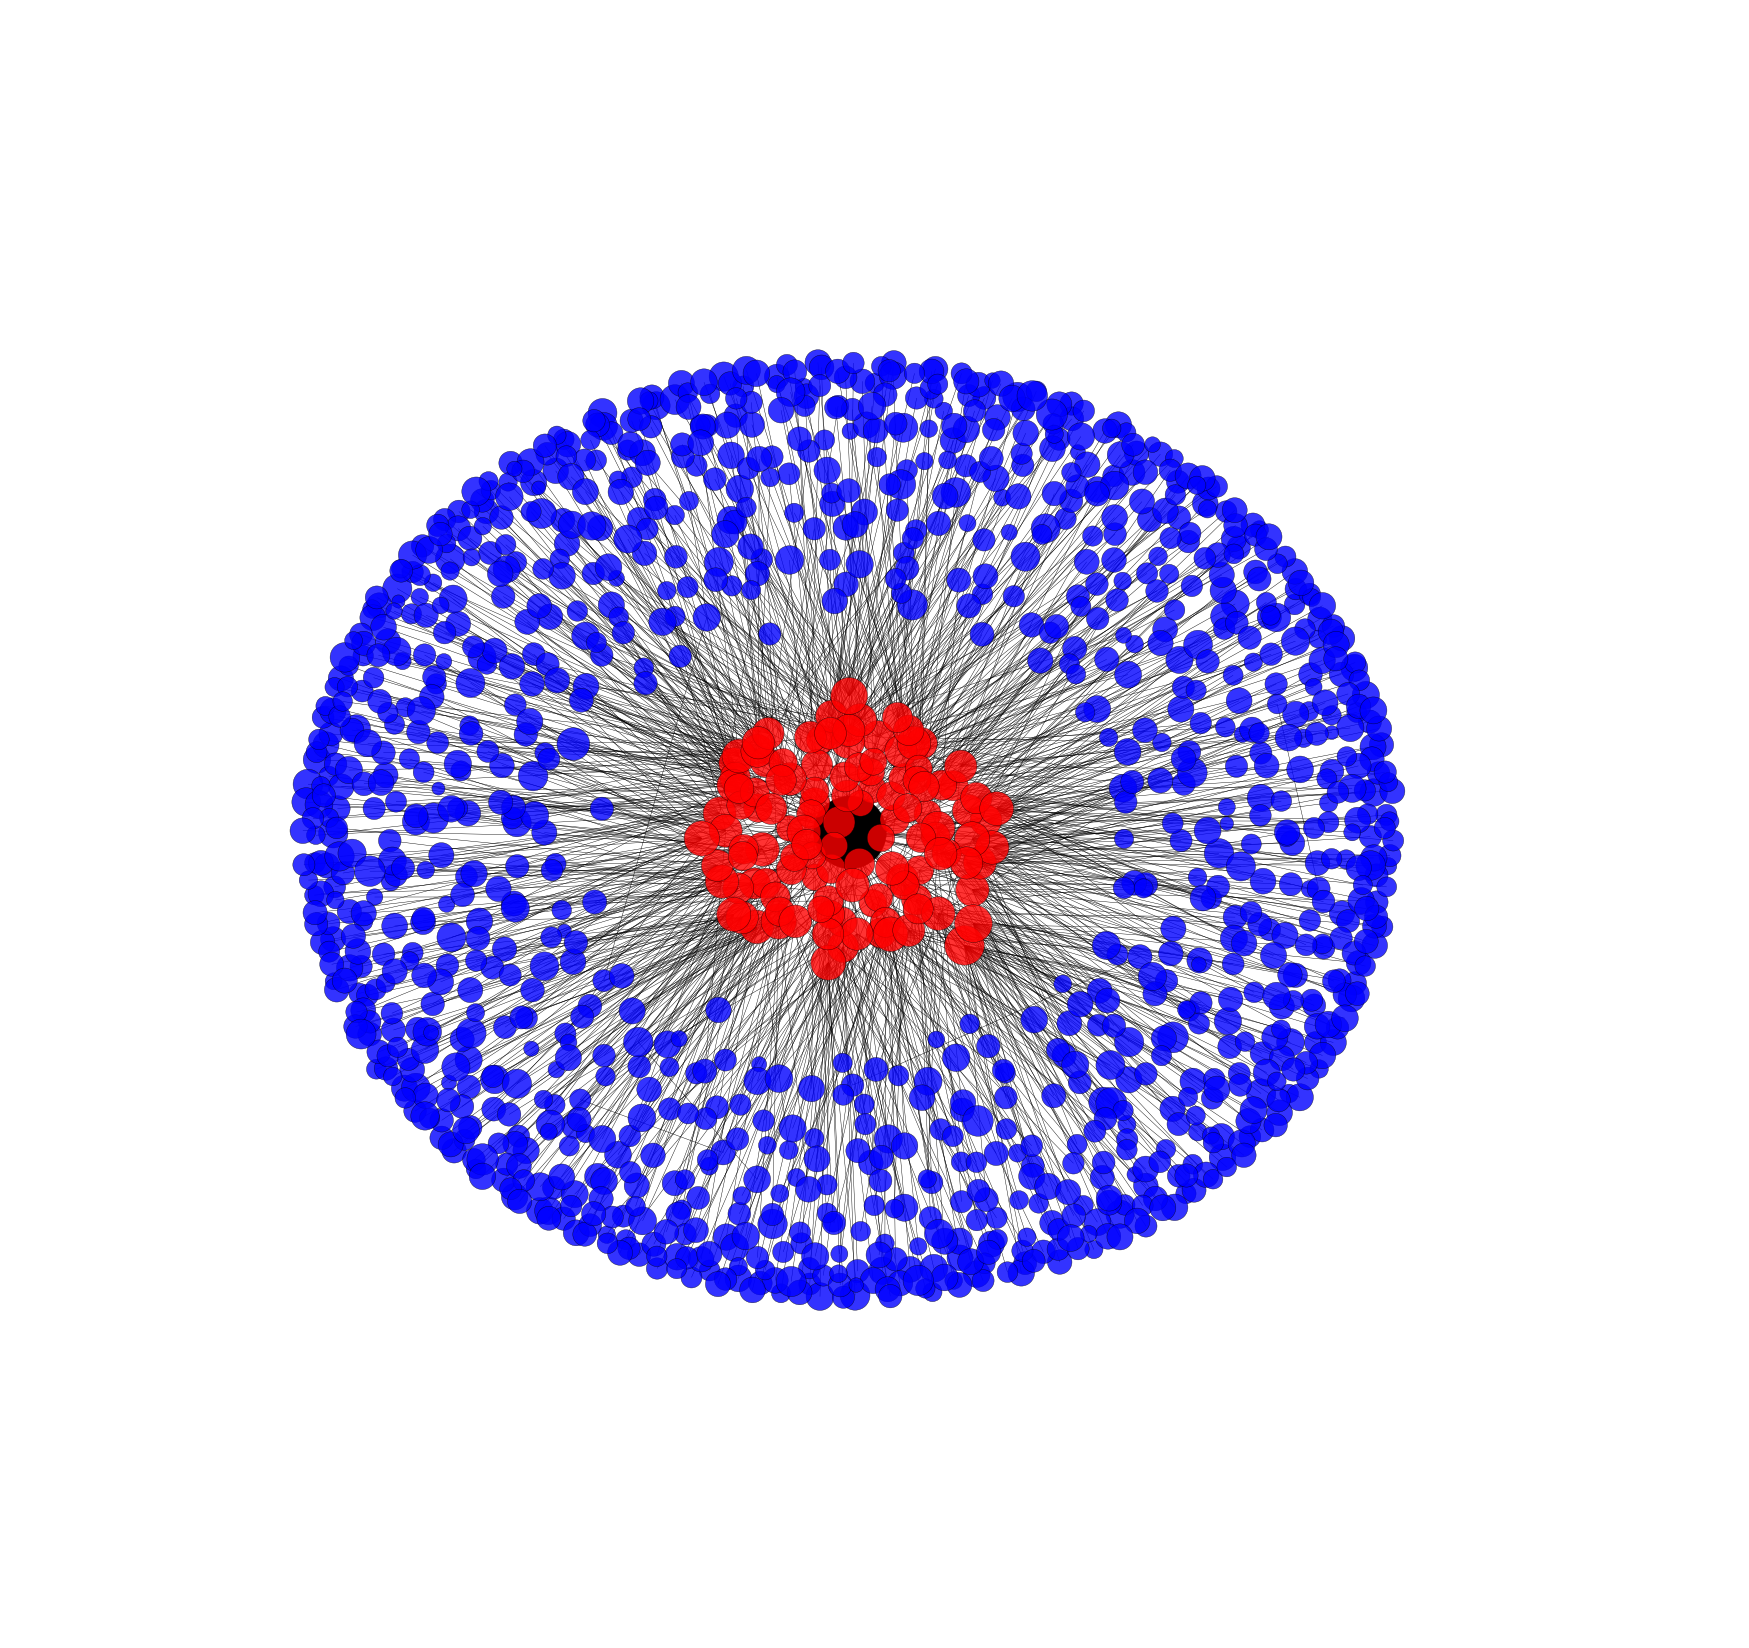
\includegraphics[width=0.49\columnwidth]{3h.png}}
\end{center}
\caption{Transition for the same Poisson random graph with growing hub size.}
\label{fig:transition}
\end{figure}

In Figure~\ref{fig:transition} we show how dramatic this can be. We show the same Poisson random graph with an added hub of size $40$, $80$, and $120$, where the area of each node is proportional to its eigenvector centrality on the left. By the third panel the eigenvalue of the hub has become the leading eigenvalue, and the hub's eigenvector centrality is much larger. The right hand side illustrates our proposed solution to this localization, non-backtracking centrality. It shows the exact same graphs, but with node size proportional to non-backtracking centrality. We see more reasonable hub behavoior in this case.

In this paper we follow Nadakuditi and Newman~\cite{nadakuditi13} and let our network be a Poisson random graph of expected degree $c$, plus a single additional hub of degree $k_n$. There is an eigenvalue corresponding to the average degree, $c+1$ and an eigenvalue corresponding to the hub, $k_n / \sqrt{k_n - c}$. We find that these cross over, and thus find a transition in the behavior of the eigenvector, when \begin{equation}\frac{k_n}{\sqrt{k_n - c}} = c+1,\end{equation} or $k_n = c(c+1)$.

After the cross over, there is localization around the hub eigenvector. The hub element is $O(1)$ and its neighbors are $O(...)$, and all other nodes are $O(...)$. We compute an order parameter to measure the degree of localization, which is:

\begin{equation}
  \omega = \sqrt[4]{\sum_i^n v_i ^ 4}
\end{equation}

$\omega$ was chosen so that the most localized eigenvector, a vector with one element equal to 1 and the rest equal to 0, gives $\omega = 1$ and the least localized eigenvector, a vector with each element $= 1/\sqrt{n}$, gives $\omega = 1/\sqrt[4]{n}$, which tends to 0 in the limit of large network size. 

Simulation results match nearly identically to the theoretical results. In Figure~\ref{fig:evalues} we see a clear crossing of eigenvalues at $k_n = 110$, as predicted. We also see a sharp phase transition in the order parameter at this point in Figure~\ref{fig:order-parameter}, as the leading eigenvector elements transition from being roughly uniform to dominated by the single element corresponding to the hub.

We also find similar results in more realistic network models. Chung~\etal~\cite{chung03} analyze the leading eigenvalue of networks generated by the configuration model with power law degree distributions of different exponents, and demonstrate a transition from an eigenvalue corresponding to the average squared degree to an eigenvalue corresponding to the square root of the maximum degree, at an exponent of $2.5$. In Figure~\ref{fig:power-law} we see this corresponds to an increase in order parameter, despite the fact that a higher power law exponent is representative of a less uniform degree distribution. This suggests that real-world networks with power-law exponent greater than 2.5 can expect localization around the largest network hub. This might affect algorithms which depend on eigenector-centrality related measures, such as PageRank.


The underlying cause of eigenvector centrality's undesirable properties is an echo chamber effect resulting from each node's centrality being influenced by its neighbors centralities. Each of the hub's neighbors obtain high centrality because they are connected to the hub, which has high centrality. The hub obtains high centrality because it has high degree, and also because it is connected to many nodes which are deemed central on account of their being connected to the hub. This amplification of centrality is what allows for extreme localization, and can be avoided by a centrality measure which takes into account neighbor centrality, but only neighbor centrality derived from nodes \emph{other than oneself}.

This concept is perfectly encapsulated by the non-backtracking matrix, or Hashimoto matrix, which has been employed and analyzed in a variety of contexts~\cite{hashimoto89,angel07,krzakala13}. The non-backtracking matrix is a $2m \times 2m$ representation of a graph in which undirected graph is turned into two directed edges, and edge $(i,j)$ is connected to every edge leaving $j$ except for its reciprocal, $(j,i)$.

This forbidding of backtracking prevents the echo chamber effect of eigenvector centrality, and solves all of the problems we've seen so far. (We analyze each of the figures and show how much more consistent it is).

We can see that non-backtracking centrality largely corresponds to eigenvector centrality. This correspondance is exact in the limit of large networks, as the one excluded edge from each edge is asymptotically negligible.

A $2m \times 2m$ matrix can be significantly larger than the original $n \times n$ adjacency matrix, and could raise concerns of intractibility. As shown in by Krzakala~\etal~\cite{krzakala13}, it is possible to compute the non-backtracking centrality of each node using only a $2n \times 2n$ matrix (show the matrix).



This centrality measure is great, but certainly not an end-all be-all. For example, it doesn't work on trees. The problem of reasonable behavior on trees has yet to be solved. We also believe there are related problems here, including belief propagation and the computation of core-periphery structure.

\begin{comment}
\begin{enumerate}
  \item Regular eigenvector centrality doesn't work.
  \begin{itemize}
	\item Introduce Hub model, talk about localization, order parameter.
	\item Give numerical results on model, real networks?
	\item Power law network theoretical results + numerics.
  \end{itemize}
  \item Hashimoto matrix
  \begin{itemize}
    \item Analytic introduction, forbidding of backtracking, echo chamber result.
    \item Tends to eigenvector centrality when dense.
    \item 2n x 2n formulation
    \item Numerical results
  \end{itemize}
  \item Doesn't work on trees, Belief Propagation / core periphery
\end{enumerate}
\end{comment}

\cite{hashimoto89, nadakuditi13, krzakala13, chung03}

\begin{figure}
\begin{center}
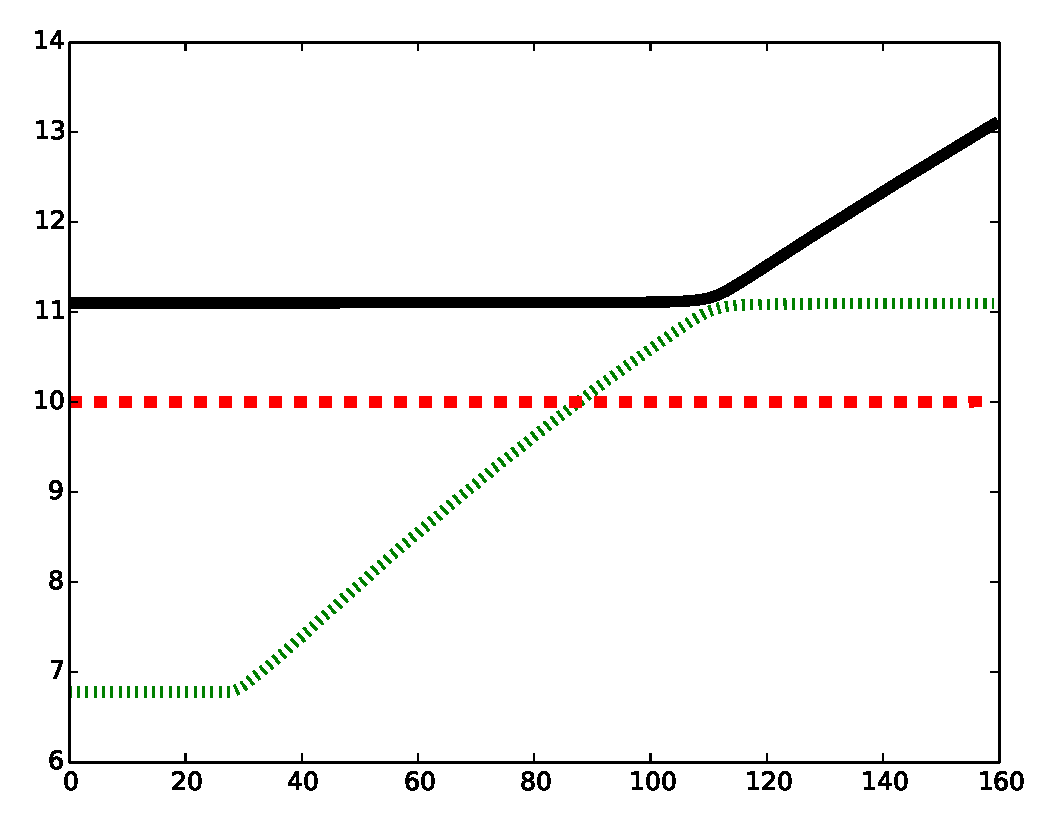
\includegraphics[width=\columnwidth]{eig.eps}
\end{center}
\caption{Eigenvalues for a graph with growing hub.}
\label{fig:evalues}
\end{figure}


\begin{figure}
\begin{center}
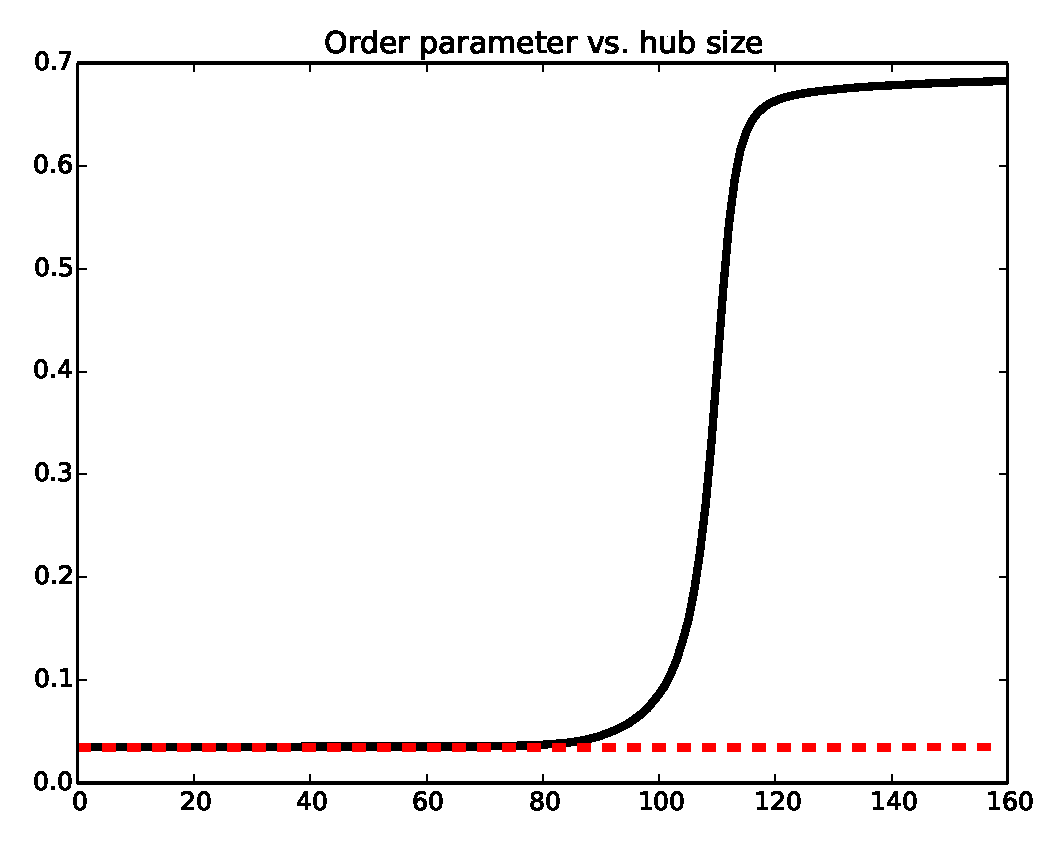
\includegraphics[width=\columnwidth]{op.eps}
\end{center}
\caption{Order parameter a graph with growing hub.}
\label{fig:order-parameter}
\end{figure}

\begin{figure}
\begin{center}
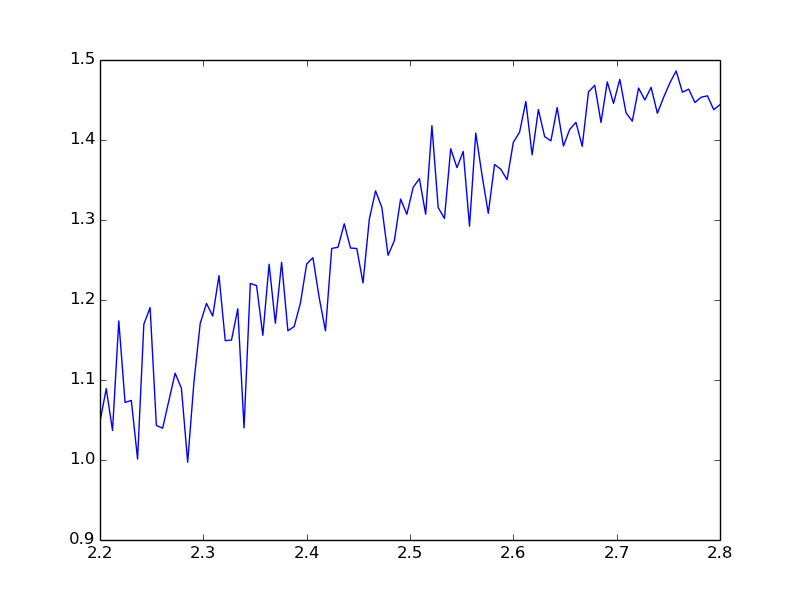
\includegraphics[width=\columnwidth]{power_plot.png}
\end{center}
\caption{Order parameter for a power law graph.}
\label{fig:power-law}
\end{figure}

\bibliography{travis}

\end{document}
